\documentclass[twoside]{book}

% Packages required by doxygen
\usepackage{fixltx2e}
\usepackage{calc}
\usepackage{doxygen}
\usepackage[export]{adjustbox} % also loads graphicx
\usepackage{graphicx}
\usepackage[utf8]{inputenc}
\usepackage{makeidx}
\usepackage{multicol}
\usepackage{multirow}
\PassOptionsToPackage{warn}{textcomp}
\usepackage{textcomp}
\usepackage[nointegrals]{wasysym}
\usepackage[table]{xcolor}

% NLS support packages
\usepackage[T2A]{fontenc}
\usepackage[russian]{babel}

% Font selection
\usepackage[T1]{fontenc}
\usepackage[scaled=.90]{helvet}
\usepackage{courier}
\usepackage{amssymb}
\usepackage{sectsty}
\renewcommand{\familydefault}{\sfdefault}
\allsectionsfont{%
  \fontseries{bc}\selectfont%
  \color{darkgray}%
}
\renewcommand{\DoxyLabelFont}{%
  \fontseries{bc}\selectfont%
  \color{darkgray}%
}
\newcommand{\+}{\discretionary{\mbox{\scriptsize$\hookleftarrow$}}{}{}}

% Page & text layout
\usepackage{geometry}
\geometry{%
  a4paper,%
  top=2.5cm,%
  bottom=2.5cm,%
  left=2.5cm,%
  right=2.5cm%
}
\tolerance=750
\hfuzz=15pt
\hbadness=750
\setlength{\emergencystretch}{15pt}
\setlength{\parindent}{0cm}
\setlength{\parskip}{3ex plus 2ex minus 2ex}
\makeatletter
\renewcommand{\paragraph}{%
  \@startsection{paragraph}{4}{0ex}{-1.0ex}{1.0ex}{%
    \normalfont\normalsize\bfseries\SS@parafont%
  }%
}
\renewcommand{\subparagraph}{%
  \@startsection{subparagraph}{5}{0ex}{-1.0ex}{1.0ex}{%
    \normalfont\normalsize\bfseries\SS@subparafont%
  }%
}
\makeatother

% Headers & footers
\usepackage{fancyhdr}
\pagestyle{fancyplain}
\fancyhead[LE]{\fancyplain{}{\bfseries\thepage}}
\fancyhead[CE]{\fancyplain{}{}}
\fancyhead[RE]{\fancyplain{}{\bfseries\leftmark}}
\fancyhead[LO]{\fancyplain{}{\bfseries\rightmark}}
\fancyhead[CO]{\fancyplain{}{}}
\fancyhead[RO]{\fancyplain{}{\bfseries\thepage}}
\fancyfoot[LE]{\fancyplain{}{}}
\fancyfoot[CE]{\fancyplain{}{}}
\fancyfoot[RE]{\fancyplain{}{\bfseries\scriptsize Создано системой Doxygen }}
\fancyfoot[LO]{\fancyplain{}{\bfseries\scriptsize Создано системой Doxygen }}
\fancyfoot[CO]{\fancyplain{}{}}
\fancyfoot[RO]{\fancyplain{}{}}
\renewcommand{\footrulewidth}{0.4pt}
\renewcommand{\chaptermark}[1]{%
  \markboth{#1}{}%
}
\renewcommand{\sectionmark}[1]{%
  \markright{\thesection\ #1}%
}

% Indices & bibliography
\usepackage{natbib}
\usepackage[titles]{tocloft}
\setcounter{tocdepth}{3}
\setcounter{secnumdepth}{5}
\makeindex

% Hyperlinks (required, but should be loaded last)
\usepackage{ifpdf}
\ifpdf
  \usepackage[pdftex,pagebackref=true]{hyperref}
\else
  \usepackage[ps2pdf,pagebackref=true]{hyperref}
\fi
\hypersetup{%
  colorlinks=true,%
  linkcolor=blue,%
  citecolor=blue,%
  unicode%
}

% Custom commands
\newcommand{\clearemptydoublepage}{%
  \newpage{\pagestyle{empty}\cleardoublepage}%
}

\usepackage{caption}
\captionsetup{labelsep=space,justification=centering,font={bf},singlelinecheck=off,skip=4pt,position=top}

%===== C O N T E N T S =====

\begin{document}

% Titlepage & ToC
\hypersetup{pageanchor=false,
             bookmarksnumbered=true,
             pdfencoding=unicode
            }
\pagenumbering{alph}
\begin{titlepage}
\vspace*{7cm}
\begin{center}%
{\Large 9Б655М симулятор \\[1ex]\large 1.\+0 }\\
\vspace*{1cm}
{\large Создано системой Doxygen 1.8.13}\\
\end{center}
\end{titlepage}
\clearemptydoublepage
\pagenumbering{roman}
\tableofcontents
\clearemptydoublepage
\pagenumbering{arabic}
\hypersetup{pageanchor=true}

%--- Begin generated contents ---
\chapter{Иерархический список классов}
\section{Иерархия классов}
Иерархия классов.\begin{DoxyCompactList}
\item \contentsline{section}{Delayer$<$ t $>$}{\pageref{classDelayer}}{}
\item \contentsline{section}{Delayer$<$ double $>$}{\pageref{classDelayer}}{}
\item \contentsline{section}{Delayer$<$ Vec3$<$ double $>$ $>$}{\pageref{classDelayer}}{}
\item \contentsline{section}{Driver}{\pageref{classDriver}}{}
\item \contentsline{section}{Exciter}{\pageref{classExciter}}{}
\item \contentsline{section}{Mean\+Filter}{\pageref{classMeanFilter}}{}
\item \contentsline{section}{Motor}{\pageref{classMotor}}{}
\begin{DoxyCompactList}
\item \contentsline{section}{Motor\+Reducer}{\pageref{classMotorReducer}}{}
\end{DoxyCompactList}
\item \contentsline{section}{Plotter}{\pageref{classPlotter}}{}
\item \contentsline{section}{quadrature\+\_\+trapez}{\pageref{classquadrature__trapez}}{}
\item \contentsline{section}{Reducer}{\pageref{classReducer}}{}
\item \contentsline{section}{Regulator}{\pageref{classRegulator}}{}
\item \contentsline{section}{Rej\+Filter}{\pageref{classRejFilter}}{}
\item \contentsline{section}{Tachometer}{\pageref{classTachometer}}{}
\item \contentsline{section}{T\+G\+A\+\_\+\+Header}{\pageref{structTGA__Header}}{}
\item \contentsline{section}{T\+G\+A\+Color}{\pageref{structTGAColor}}{}
\item \contentsline{section}{T\+G\+A\+Image}{\pageref{classTGAImage}}{}
\item \contentsline{section}{Vec3$<$ T $>$}{\pageref{structVec3}}{}
\item \contentsline{section}{Vec3$<$ double $>$}{\pageref{structVec3}}{}
\item \contentsline{section}{Vector\+Controller}{\pageref{classVectorController}}{}
\end{DoxyCompactList}

\chapter{Алфавитный указатель классов}
\section{Классы}
Классы с их кратким описанием.\begin{DoxyCompactList}
\item\contentsline{section}{\hyperlink{classDelayer}{Delayer$<$ t $>$} \\*Класс линии задержки }{\pageref{classDelayer}}{}
\item\contentsline{section}{\hyperlink{classDriver}{Driver} \\*Класс одногоканального привода }{\pageref{classDriver}}{}
\item\contentsline{section}{\hyperlink{classExciter}{Exciter} \\*Класс трехфазного источника напряжения }{\pageref{classExciter}}{}
\item\contentsline{section}{\hyperlink{classMeanFilter}{Mean\+Filter} \\*Класс цифрового усредняющего фильтра }{\pageref{classMeanFilter}}{}
\item\contentsline{section}{\hyperlink{classMotor}{Motor} \\*Класс синхронного электродвигателя }{\pageref{classMotor}}{}
\item\contentsline{section}{\hyperlink{classMotorReducer}{Motor\+Reducer} \\*Класс синхронного электродвигателя для использования с редуктором }{\pageref{classMotorReducer}}{}
\item\contentsline{section}{\hyperlink{classPlotter}{Plotter} \\*Класс построителя 2D диаграмм }{\pageref{classPlotter}}{}
\item\contentsline{section}{\hyperlink{classquadrature__trapez}{quadrature\+\_\+trapez} \\*Класс численного вычисления квадратур методом трапеций }{\pageref{classquadrature__trapez}}{}
\item\contentsline{section}{\hyperlink{classReducer}{Reducer} \\*Класс линейного редуктора }{\pageref{classReducer}}{}
\item\contentsline{section}{\hyperlink{classRegulator}{Regulator} \\*Класс ПИ регулятора }{\pageref{classRegulator}}{}
\item\contentsline{section}{\hyperlink{classRejFilter}{Rej\+Filter} \\*Класс цифрового режекторнорго фильтра }{\pageref{classRejFilter}}{}
\item\contentsline{section}{\hyperlink{classTachometer}{Tachometer} \\*Класс измерителя скорости вращения ротора }{\pageref{classTachometer}}{}
\item\contentsline{section}{\hyperlink{structTGA__Header}{T\+G\+A\+\_\+\+Header} \\*Класс для работы с tga изображениями }{\pageref{structTGA__Header}}{}
\item\contentsline{section}{\hyperlink{structTGAColor}{T\+G\+A\+Color} \\*Класс для работы с tga изображениями }{\pageref{structTGAColor}}{}
\item\contentsline{section}{\hyperlink{classTGAImage}{T\+G\+A\+Image} \\*Класс для работы с tga изображениями }{\pageref{classTGAImage}}{}
\item\contentsline{section}{\hyperlink{structVec3}{Vec3$<$ T $>$} \\*Класс 3D вектора }{\pageref{structVec3}}{}
\item\contentsline{section}{\hyperlink{classVectorController}{Vector\+Controller} \\*Класс векторного контроллера }{\pageref{classVectorController}}{}
\end{DoxyCompactList}

\chapter{Список файлов}
\section{Файлы}
Полный список документированных файлов.\begin{DoxyCompactList}
\item\contentsline{section}{\hyperlink{config_8h}{config.\+h} }{\pageref{config_8h}}{}
\item\contentsline{section}{{\bfseries controller.\+h} }{\pageref{controller_8h}}{}
\item\contentsline{section}{{\bfseries cos\+\_\+tb.\+h} }{\pageref{cos__tb_8h}}{}
\item\contentsline{section}{{\bfseries delayer.\+h} }{\pageref{delayer_8h}}{}
\item\contentsline{section}{{\bfseries driver.\+h} }{\pageref{driver_8h}}{}
\item\contentsline{section}{{\bfseries exciter.\+h} }{\pageref{exciter_8h}}{}
\item\contentsline{section}{{\bfseries filter.\+h} }{\pageref{filter_8h}}{}
\item\contentsline{section}{\hyperlink{gdef_8h}{gdef.\+h} }{\pageref{gdef_8h}}{}
\item\contentsline{section}{{\bfseries geometry.\+h} }{\pageref{geometry_8h}}{}
\item\contentsline{section}{{\bfseries motor.\+h} }{\pageref{motor_8h}}{}
\item\contentsline{section}{{\bfseries plotter.\+h} }{\pageref{plotter_8h}}{}
\item\contentsline{section}{{\bfseries reducer.\+h} }{\pageref{reducer_8h}}{}
\item\contentsline{section}{{\bfseries regulator.\+h} }{\pageref{regulator_8h}}{}
\item\contentsline{section}{{\bfseries tachometer.\+h} }{\pageref{tachometer_8h}}{}
\item\contentsline{section}{{\bfseries tgaimage.\+h} }{\pageref{tgaimage_8h}}{}
\end{DoxyCompactList}

\chapter{Классы}
\hypertarget{classDelayer}{}\section{Шаблон класса Delayer$<$ t $>$}
\label{classDelayer}\index{Delayer$<$ t $>$@{Delayer$<$ t $>$}}


Класс линии задержки  




{\ttfamily \#include $<$delayer.\+h$>$}

\subsection*{Открытые члены}
\begin{DoxyCompactItemize}
\item 
\mbox{\Hypertarget{classDelayer_a24010c6b64b225c6255f2109ba143e22}\label{classDelayer_a24010c6b64b225c6255f2109ba143e22}} 
{\bfseries Delayer} (int n)
\item 
t \hyperlink{classDelayer_a7aafed93e61eb191c02fa841728d63de}{operator()} (t x)
\begin{DoxyCompactList}\small\item\em обновляет состояние \end{DoxyCompactList}\end{DoxyCompactItemize}


\subsection{Подробное описание}
\subsubsection*{template$<$class t$>$\newline
class Delayer$<$ t $>$}

Класс линии задержки 

\subsection{Методы}
\mbox{\Hypertarget{classDelayer_a7aafed93e61eb191c02fa841728d63de}\label{classDelayer_a7aafed93e61eb191c02fa841728d63de}} 
\index{Delayer@{Delayer}!operator()@{operator()}}
\index{operator()@{operator()}!Delayer@{Delayer}}
\subsubsection{\texorpdfstring{operator()()}{operator()()}}
{\footnotesize\ttfamily template$<$class t$>$ \\
t \hyperlink{classDelayer}{Delayer}$<$ t $>$\+::operator() (\begin{DoxyParamCaption}\item[{t}]{x }\end{DoxyParamCaption})\hspace{0.3cm}{\ttfamily [inline]}}



обновляет состояние 


\begin{DoxyParams}{Аргументы}
{\em x} & текущее значение элемента \\
\hline
\end{DoxyParams}
\begin{DoxyReturn}{Возвращает}
элемент задержанный на n тактов 
\end{DoxyReturn}


Объявления и описания членов класса находятся в файле\+:\begin{DoxyCompactItemize}
\item 
delayer.\+h\end{DoxyCompactItemize}

\hypertarget{classDriver}{}\section{Класс Driver}
\label{classDriver}\index{Driver@{Driver}}


Класс одногоканального привода  




{\ttfamily \#include $<$driver.\+h$>$}

\subsection*{Открытые члены}
\begin{DoxyCompactItemize}
\item 
\hyperlink{classDriver_a62215da042c694ceea51b2d65605db1f}{Driver} (double \+\_\+dt)
\item 
\hyperlink{structVec3}{Vec3d} \hyperlink{classDriver_a15e3c21483960b7a7af260273e95f294}{operator()} (double ux)
\end{DoxyCompactItemize}


\subsection{Подробное описание}
Класс одногоканального привода 

\subsection{Конструктор(ы)}
\mbox{\Hypertarget{classDriver_a62215da042c694ceea51b2d65605db1f}\label{classDriver_a62215da042c694ceea51b2d65605db1f}} 
\index{Driver@{Driver}!Driver@{Driver}}
\index{Driver@{Driver}!Driver@{Driver}}
\subsubsection{\texorpdfstring{Driver()}{Driver()}}
{\footnotesize\ttfamily Driver\+::\+Driver (\begin{DoxyParamCaption}\item[{double}]{\+\_\+dt }\end{DoxyParamCaption})\hspace{0.3cm}{\ttfamily [inline]}}


\begin{DoxyParams}{Аргументы}
{\em \+\_\+dt} & Шаг интегрирования \\
\hline
\end{DoxyParams}


\subsection{Методы}
\mbox{\Hypertarget{classDriver_a15e3c21483960b7a7af260273e95f294}\label{classDriver_a15e3c21483960b7a7af260273e95f294}} 
\index{Driver@{Driver}!operator()@{operator()}}
\index{operator()@{operator()}!Driver@{Driver}}
\subsubsection{\texorpdfstring{operator()()}{operator()()}}
{\footnotesize\ttfamily \hyperlink{structVec3}{Vec3d} Driver\+::operator() (\begin{DoxyParamCaption}\item[{double}]{ux }\end{DoxyParamCaption})\hspace{0.3cm}{\ttfamily [inline]}}


\begin{DoxyParams}{Аргументы}
{\em ux} & напряжение уставки регулятора положения -\/10В..+10В \\
\hline
\end{DoxyParams}
\begin{DoxyReturn}{Возвращает}
вектор состояния -\/ (положение м, скорость м/с, усилие на штоке Н) 
\end{DoxyReturn}


Объявления и описания членов класса находятся в файле\+:\begin{DoxyCompactItemize}
\item 
driver.\+h\end{DoxyCompactItemize}

\hypertarget{classExciter}{}\section{Класс Exciter}
\label{classExciter}\index{Exciter@{Exciter}}


Класс трехфазного источника напряжения  




{\ttfamily \#include $<$exciter.\+h$>$}



Граф связей класса Exciter\+:\nopagebreak
\begin{figure}[H]
\begin{center}
\leavevmode
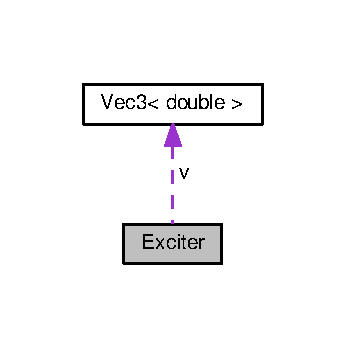
\includegraphics[width=166pt]{classExciter__coll__graph}
\end{center}
\end{figure}
\subsection*{Открытые члены}
\begin{DoxyCompactItemize}
\item 
\hyperlink{classExciter_a4d33a218b5cafd84cd55c8b51cd9246d}{Exciter} (double a, double f)
\item 
\hyperlink{structVec3}{Vec3d} \hyperlink{classExciter_a7dae2402806160fd5b7a12e9088b6c05}{operator()} (double t)
\begin{DoxyCompactList}\small\item\em обновляет состояние \end{DoxyCompactList}\end{DoxyCompactItemize}
\subsection*{Открытые атрибуты}
\begin{DoxyCompactItemize}
\item 
\mbox{\Hypertarget{classExciter_a62ae9d6c77ca3876158db3405ccb0522}\label{classExciter_a62ae9d6c77ca3876158db3405ccb0522}} 
\hyperlink{structVec3}{Vec3d} {\bfseries v}
\end{DoxyCompactItemize}


\subsection{Подробное описание}
Класс трехфазного источника напряжения 

\subsection{Конструктор(ы)}
\mbox{\Hypertarget{classExciter_a4d33a218b5cafd84cd55c8b51cd9246d}\label{classExciter_a4d33a218b5cafd84cd55c8b51cd9246d}} 
\index{Exciter@{Exciter}!Exciter@{Exciter}}
\index{Exciter@{Exciter}!Exciter@{Exciter}}
\subsubsection{\texorpdfstring{Exciter()}{Exciter()}}
{\footnotesize\ttfamily Exciter\+::\+Exciter (\begin{DoxyParamCaption}\item[{double}]{a,  }\item[{double}]{f }\end{DoxyParamCaption})\hspace{0.3cm}{\ttfamily [inline]}}


\begin{DoxyParams}{Аргументы}
{\em a} & амплитуда В \\
\hline
{\em f} & частота Гц \\
\hline
\end{DoxyParams}


\subsection{Методы}
\mbox{\Hypertarget{classExciter_a7dae2402806160fd5b7a12e9088b6c05}\label{classExciter_a7dae2402806160fd5b7a12e9088b6c05}} 
\index{Exciter@{Exciter}!operator()@{operator()}}
\index{operator()@{operator()}!Exciter@{Exciter}}
\subsubsection{\texorpdfstring{operator()()}{operator()()}}
{\footnotesize\ttfamily \hyperlink{structVec3}{Vec3d} Exciter\+::operator() (\begin{DoxyParamCaption}\item[{double}]{t }\end{DoxyParamCaption})\hspace{0.3cm}{\ttfamily [inline]}}



обновляет состояние 


\begin{DoxyParams}{Аргументы}
{\em t} & текущее время \\
\hline
\end{DoxyParams}
\begin{DoxyReturn}{Возвращает}
вектор фазных напряжений 
\end{DoxyReturn}


Объявления и описания членов класса находятся в файле\+:\begin{DoxyCompactItemize}
\item 
exciter.\+h\end{DoxyCompactItemize}

\hypertarget{classMeanFilter}{}\section{Класс Mean\+Filter}
\label{classMeanFilter}\index{Mean\+Filter@{Mean\+Filter}}


Класс цифрового усредняющего фильтра  




{\ttfamily \#include $<$filter.\+h$>$}

\subsection*{Открытые члены}
\begin{DoxyCompactItemize}
\item 
\mbox{\Hypertarget{classMeanFilter_ae3c9f665fde03a41a994ca509d9862af}\label{classMeanFilter_ae3c9f665fde03a41a994ca509d9862af}} 
{\bfseries Mean\+Filter} (int32\+\_\+t ord)
\item 
\mbox{\Hypertarget{classMeanFilter_a5f6eabe16c6bbf4266a7d2a9b188b0c5}\label{classMeanFilter_a5f6eabe16c6bbf4266a7d2a9b188b0c5}} 
int32\+\_\+t {\bfseries operator()} (int32\+\_\+t x)
\end{DoxyCompactItemize}


\subsection{Подробное описание}
Класс цифрового усредняющего фильтра 

Объявления и описания членов класса находятся в файле\+:\begin{DoxyCompactItemize}
\item 
filter.\+h\end{DoxyCompactItemize}

\hypertarget{classMotor}{}\section{Класс Motor}
\label{classMotor}\index{Motor@{Motor}}


Класс синхронного электродвигателя  




{\ttfamily \#include $<$motor.\+h$>$}



Граф наследования\+:Motor\+:\nopagebreak
\begin{figure}[H]
\begin{center}
\leavevmode
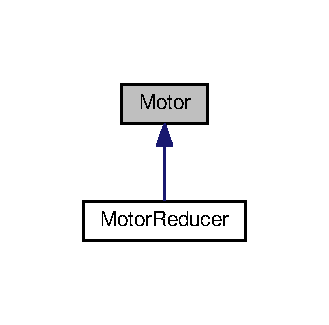
\includegraphics[width=158pt]{classMotor__inherit__graph}
\end{center}
\end{figure}
\subsection*{Открытые члены}
\begin{DoxyCompactItemize}
\item 
\hyperlink{classMotor_a060931682af482a7f7b1169304cbcd52}{Motor} (double t)
\item 
double \hyperlink{classMotor_a30091b07e2c1aa8d85047f84e3137c79}{operator()} (const \hyperlink{structVec3}{Vec3d} \&vex, double load)
\begin{DoxyCompactList}\small\item\em обновляет состояние \end{DoxyCompactList}\item 
\hyperlink{structVec3}{Vec3d} \hyperlink{classMotor_a55899b432198761a45182151c5817df1}{getstate} ()
\item 
\hyperlink{structVec3}{Vec3d} \hyperlink{classMotor_a519cb1cf6fd48ce81f718eb340bbe9df}{getcurr} ()
\item 
double \hyperlink{classMotor_aced401ab0a40ead568739392cea51748}{getspd} ()
\item 
double \hyperlink{classMotor_a2252f262ca385e6a1ae217c9f2f9d282}{getpos} ()
\item 
double \hyperlink{classMotor_ac14e02e5c16a5ffe35815fe2bf586fbe}{gettorque} ()
\end{DoxyCompactItemize}
\subsection*{Друзья}
\begin{DoxyCompactItemize}
\item 
\mbox{\Hypertarget{classMotor_a6de8620f6da17a10dd96a51dad28b54f}\label{classMotor_a6de8620f6da17a10dd96a51dad28b54f}} 
std\+::ostream \& {\bfseries operator$<$$<$} (std\+::ostream \&s, \hyperlink{classMotor}{Motor} \&m)
\end{DoxyCompactItemize}


\subsection{Подробное описание}
Класс синхронного электродвигателя 

\subsection{Конструктор(ы)}
\mbox{\Hypertarget{classMotor_a060931682af482a7f7b1169304cbcd52}\label{classMotor_a060931682af482a7f7b1169304cbcd52}} 
\index{Motor@{Motor}!Motor@{Motor}}
\index{Motor@{Motor}!Motor@{Motor}}
\subsubsection{\texorpdfstring{Motor()}{Motor()}}
{\footnotesize\ttfamily Motor\+::\+Motor (\begin{DoxyParamCaption}\item[{double}]{t }\end{DoxyParamCaption})\hspace{0.3cm}{\ttfamily [inline]}}


\begin{DoxyParams}{Аргументы}
{\em t} & шаг интегрирования \\
\hline
\end{DoxyParams}


\subsection{Методы}
\mbox{\Hypertarget{classMotor_a519cb1cf6fd48ce81f718eb340bbe9df}\label{classMotor_a519cb1cf6fd48ce81f718eb340bbe9df}} 
\index{Motor@{Motor}!getcurr@{getcurr}}
\index{getcurr@{getcurr}!Motor@{Motor}}
\subsubsection{\texorpdfstring{getcurr()}{getcurr()}}
{\footnotesize\ttfamily \hyperlink{structVec3}{Vec3d} Motor\+::getcurr (\begin{DoxyParamCaption}{ }\end{DoxyParamCaption})\hspace{0.3cm}{\ttfamily [inline]}}

\begin{DoxyReturn}{Возвращает}
вектор фазных токов А 
\end{DoxyReturn}
\mbox{\Hypertarget{classMotor_a2252f262ca385e6a1ae217c9f2f9d282}\label{classMotor_a2252f262ca385e6a1ae217c9f2f9d282}} 
\index{Motor@{Motor}!getpos@{getpos}}
\index{getpos@{getpos}!Motor@{Motor}}
\subsubsection{\texorpdfstring{getpos()}{getpos()}}
{\footnotesize\ttfamily double Motor\+::getpos (\begin{DoxyParamCaption}{ }\end{DoxyParamCaption})\hspace{0.3cm}{\ttfamily [inline]}}

\begin{DoxyReturn}{Возвращает}
угловое положение ротора рад 
\end{DoxyReturn}
\mbox{\Hypertarget{classMotor_aced401ab0a40ead568739392cea51748}\label{classMotor_aced401ab0a40ead568739392cea51748}} 
\index{Motor@{Motor}!getspd@{getspd}}
\index{getspd@{getspd}!Motor@{Motor}}
\subsubsection{\texorpdfstring{getspd()}{getspd()}}
{\footnotesize\ttfamily double Motor\+::getspd (\begin{DoxyParamCaption}{ }\end{DoxyParamCaption})\hspace{0.3cm}{\ttfamily [inline]}}

\begin{DoxyReturn}{Возвращает}
угловая скорость рад/с 
\end{DoxyReturn}
\mbox{\Hypertarget{classMotor_a55899b432198761a45182151c5817df1}\label{classMotor_a55899b432198761a45182151c5817df1}} 
\index{Motor@{Motor}!getstate@{getstate}}
\index{getstate@{getstate}!Motor@{Motor}}
\subsubsection{\texorpdfstring{getstate()}{getstate()}}
{\footnotesize\ttfamily \hyperlink{structVec3}{Vec3d} Motor\+::getstate (\begin{DoxyParamCaption}{ }\end{DoxyParamCaption})\hspace{0.3cm}{\ttfamily [inline]}}

\begin{DoxyReturn}{Возвращает}
вектор состояния двигателя (угловое положение ротора рад, угловая скорость рад/c, ускорение рад/c2) 
\end{DoxyReturn}
\mbox{\Hypertarget{classMotor_ac14e02e5c16a5ffe35815fe2bf586fbe}\label{classMotor_ac14e02e5c16a5ffe35815fe2bf586fbe}} 
\index{Motor@{Motor}!gettorque@{gettorque}}
\index{gettorque@{gettorque}!Motor@{Motor}}
\subsubsection{\texorpdfstring{gettorque()}{gettorque()}}
{\footnotesize\ttfamily double Motor\+::gettorque (\begin{DoxyParamCaption}{ }\end{DoxyParamCaption})\hspace{0.3cm}{\ttfamily [inline]}}

\begin{DoxyReturn}{Возвращает}
момент развиваемый двигателем Н$\ast$м 
\end{DoxyReturn}
\mbox{\Hypertarget{classMotor_a30091b07e2c1aa8d85047f84e3137c79}\label{classMotor_a30091b07e2c1aa8d85047f84e3137c79}} 
\index{Motor@{Motor}!operator()@{operator()}}
\index{operator()@{operator()}!Motor@{Motor}}
\subsubsection{\texorpdfstring{operator()()}{operator()()}}
{\footnotesize\ttfamily double Motor\+::operator() (\begin{DoxyParamCaption}\item[{const \hyperlink{structVec3}{Vec3d} \&}]{vex,  }\item[{double}]{load }\end{DoxyParamCaption})\hspace{0.3cm}{\ttfamily [inline]}}



обновляет состояние 


\begin{DoxyParams}{Аргументы}
{\em vex} & вектор фазных напряжений \\
\hline
{\em load} & нагружающий момент Н$\ast$м \\
\hline
\end{DoxyParams}
\begin{DoxyReturn}{Возвращает}
момент развиваемый двигателем 
\end{DoxyReturn}


Объявления и описания членов класса находятся в файле\+:\begin{DoxyCompactItemize}
\item 
motor.\+h\end{DoxyCompactItemize}

\hypertarget{classMotorReducer}{}\section{Класс Motor\+Reducer}
\label{classMotorReducer}\index{Motor\+Reducer@{Motor\+Reducer}}


Класс синхронного электродвигателя для использования с редуктором  




{\ttfamily \#include $<$motor.\+h$>$}



Граф наследования\+:Motor\+Reducer\+:\nopagebreak
\begin{figure}[H]
\begin{center}
\leavevmode
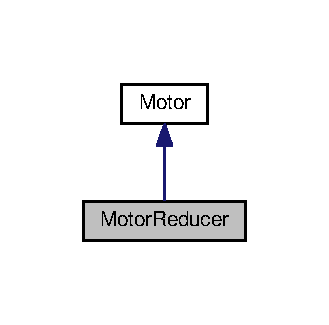
\includegraphics[width=158pt]{classMotorReducer__inherit__graph}
\end{center}
\end{figure}


Граф связей класса Motor\+Reducer\+:\nopagebreak
\begin{figure}[H]
\begin{center}
\leavevmode
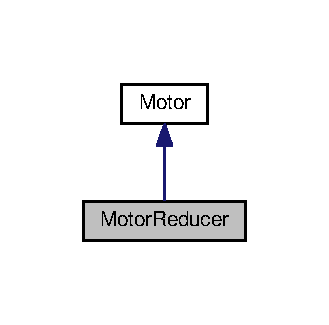
\includegraphics[width=158pt]{classMotorReducer__coll__graph}
\end{center}
\end{figure}
\subsection*{Открытые члены}
\begin{DoxyCompactItemize}
\item 
\hyperlink{classMotorReducer_a85ac4fe9831900c6697ee80ff0cc3d32}{Motor\+Reducer} (double dt)
\item 
double \hyperlink{classMotorReducer_a29141a375c33d409928f40962fcd4011}{operator()} (const \hyperlink{structVec3}{Vec3d} \&vex, double spd)
\begin{DoxyCompactList}\small\item\em обновляет состояние \end{DoxyCompactList}\end{DoxyCompactItemize}


\subsection{Подробное описание}
Класс синхронного электродвигателя для использования с редуктором 

\subsection{Конструктор(ы)}
\mbox{\Hypertarget{classMotorReducer_a85ac4fe9831900c6697ee80ff0cc3d32}\label{classMotorReducer_a85ac4fe9831900c6697ee80ff0cc3d32}} 
\index{Motor\+Reducer@{Motor\+Reducer}!Motor\+Reducer@{Motor\+Reducer}}
\index{Motor\+Reducer@{Motor\+Reducer}!Motor\+Reducer@{Motor\+Reducer}}
\subsubsection{\texorpdfstring{Motor\+Reducer()}{MotorReducer()}}
{\footnotesize\ttfamily Motor\+Reducer\+::\+Motor\+Reducer (\begin{DoxyParamCaption}\item[{double}]{dt }\end{DoxyParamCaption})\hspace{0.3cm}{\ttfamily [inline]}}


\begin{DoxyParams}{Аргументы}
{\em t} & шаг интегрирования \\
\hline
\end{DoxyParams}


\subsection{Методы}
\mbox{\Hypertarget{classMotorReducer_a29141a375c33d409928f40962fcd4011}\label{classMotorReducer_a29141a375c33d409928f40962fcd4011}} 
\index{Motor\+Reducer@{Motor\+Reducer}!operator()@{operator()}}
\index{operator()@{operator()}!Motor\+Reducer@{Motor\+Reducer}}
\subsubsection{\texorpdfstring{operator()()}{operator()()}}
{\footnotesize\ttfamily double Motor\+Reducer\+::operator() (\begin{DoxyParamCaption}\item[{const \hyperlink{structVec3}{Vec3d} \&}]{vex,  }\item[{double}]{spd }\end{DoxyParamCaption})\hspace{0.3cm}{\ttfamily [inline]}}



обновляет состояние 


\begin{DoxyParams}{Аргументы}
{\em vex} & вектор фазных напряжений \\
\hline
{\em spd} & угловая скорость ротора рад/c \\
\hline
\end{DoxyParams}
\begin{DoxyReturn}{Возвращает}
момент развиваемый двигателем 
\end{DoxyReturn}


Объявления и описания членов класса находятся в файле\+:\begin{DoxyCompactItemize}
\item 
motor.\+h\end{DoxyCompactItemize}

\hypertarget{classPlotter}{}\section{Класс Plotter}
\label{classPlotter}\index{Plotter@{Plotter}}


Класс построителя 2D диаграмм  




{\ttfamily \#include $<$plotter.\+h$>$}

\subsection*{Открытые члены}
\begin{DoxyCompactItemize}
\item 
\mbox{\Hypertarget{classPlotter_a7d399312dc9083c9c7867908ab09dab2}\label{classPlotter_a7d399312dc9083c9c7867908ab09dab2}} 
{\bfseries Plotter} (const std\+::string fn, const double xsc, const \hyperlink{structVec3}{Vec3d} ysc)
\item 
\mbox{\Hypertarget{classPlotter_a5abb01053eab3962b30c78a3db678e22}\label{classPlotter_a5abb01053eab3962b30c78a3db678e22}} 
void {\bfseries operator()} (const \hyperlink{structVec3}{Vec3d} \&y, const double x)
\item 
\mbox{\Hypertarget{classPlotter_a2a6c933fd57331a7643592b5e140d3ce}\label{classPlotter_a2a6c933fd57331a7643592b5e140d3ce}} 
void {\bfseries line} (int x0, int y0, int x1, int y1, \hyperlink{structTGAColor}{T\+G\+A\+Color} color)
\end{DoxyCompactItemize}


\subsection{Подробное описание}
Класс построителя 2D диаграмм 

Объявления и описания членов классов находятся в файлах\+:\begin{DoxyCompactItemize}
\item 
plotter.\+h\item 
plotter.\+cpp\end{DoxyCompactItemize}

\hypertarget{classquadrature__trapez}{}\section{Класс quadrature\+\_\+trapez}
\label{classquadrature__trapez}\index{quadrature\+\_\+trapez@{quadrature\+\_\+trapez}}


Класс численного вычисления квадратур методом трапеций  




{\ttfamily \#include $<$geometry.\+h$>$}

\subsection*{Открытые члены}
\begin{DoxyCompactItemize}
\item 
\mbox{\Hypertarget{classquadrature__trapez_ae0ccaaa6f535addd5e2f590288905be6}\label{classquadrature__trapez_ae0ccaaa6f535addd5e2f590288905be6}} 
{\bfseries quadrature\+\_\+trapez} (double dt)
\item 
\mbox{\Hypertarget{classquadrature__trapez_a53e90bc96e1e4e2522f9d462287f9cee}\label{classquadrature__trapez_a53e90bc96e1e4e2522f9d462287f9cee}} 
double {\bfseries operator()} (double x)
\item 
\mbox{\Hypertarget{classquadrature__trapez_ab3fb522d3ce115635fe560e86bb7ae20}\label{classquadrature__trapez_ab3fb522d3ce115635fe560e86bb7ae20}} 
double {\bfseries operator()} (double x, bool fs)
\end{DoxyCompactItemize}


\subsection{Подробное описание}
Класс численного вычисления квадратур методом трапеций 

Объявления и описания членов класса находятся в файле\+:\begin{DoxyCompactItemize}
\item 
geometry.\+h\end{DoxyCompactItemize}

\hypertarget{classReducer}{}\section{Класс Reducer}
\label{classReducer}\index{Reducer@{Reducer}}


Класс линейного редуктора  




{\ttfamily \#include $<$reducer.\+h$>$}

\subsection*{Открытые члены}
\begin{DoxyCompactItemize}
\item 
\hyperlink{classReducer_aef34e959e4ee8b88409b550245caf460}{Reducer} (double t)
\item 
double \hyperlink{classReducer_a2ba34bd1a838b483352560f568251a17}{operator()} (double Mdv)
\begin{DoxyCompactList}\small\item\em обновляет состояние \end{DoxyCompactList}\item 
\hyperlink{structVec3}{Vec3d} \hyperlink{classReducer_a758fff1ae35351c70fdbefec4b796105}{getstate} ()
\end{DoxyCompactItemize}
\subsection*{Друзья}
\begin{DoxyCompactItemize}
\item 
\mbox{\Hypertarget{classReducer_ad45359cd93ad74e5957c630e8d559bda}\label{classReducer_ad45359cd93ad74e5957c630e8d559bda}} 
std\+::ostream \& {\bfseries operator$<$$<$} (std\+::ostream \&s, \hyperlink{classReducer}{Reducer} \&r)
\end{DoxyCompactItemize}


\subsection{Подробное описание}
Класс линейного редуктора 

\subsection{Конструктор(ы)}
\mbox{\Hypertarget{classReducer_aef34e959e4ee8b88409b550245caf460}\label{classReducer_aef34e959e4ee8b88409b550245caf460}} 
\index{Reducer@{Reducer}!Reducer@{Reducer}}
\index{Reducer@{Reducer}!Reducer@{Reducer}}
\subsubsection{\texorpdfstring{Reducer()}{Reducer()}}
{\footnotesize\ttfamily Reducer\+::\+Reducer (\begin{DoxyParamCaption}\item[{double}]{t }\end{DoxyParamCaption})\hspace{0.3cm}{\ttfamily [inline]}}


\begin{DoxyParams}{Аргументы}
{\em t} & шаг интегрирования \\
\hline
\end{DoxyParams}


\subsection{Методы}
\mbox{\Hypertarget{classReducer_a758fff1ae35351c70fdbefec4b796105}\label{classReducer_a758fff1ae35351c70fdbefec4b796105}} 
\index{Reducer@{Reducer}!getstate@{getstate}}
\index{getstate@{getstate}!Reducer@{Reducer}}
\subsubsection{\texorpdfstring{getstate()}{getstate()}}
{\footnotesize\ttfamily \hyperlink{structVec3}{Vec3d} Reducer\+::getstate (\begin{DoxyParamCaption}{ }\end{DoxyParamCaption})\hspace{0.3cm}{\ttfamily [inline]}}

\begin{DoxyReturn}{Возвращает}
вектор состояния редуктора (положение м, скорость м/с, усилие на штоке Н) 
\end{DoxyReturn}
\mbox{\Hypertarget{classReducer_a2ba34bd1a838b483352560f568251a17}\label{classReducer_a2ba34bd1a838b483352560f568251a17}} 
\index{Reducer@{Reducer}!operator()@{operator()}}
\index{operator()@{operator()}!Reducer@{Reducer}}
\subsubsection{\texorpdfstring{operator()()}{operator()()}}
{\footnotesize\ttfamily double Reducer\+::operator() (\begin{DoxyParamCaption}\item[{double}]{Mdv }\end{DoxyParamCaption})\hspace{0.3cm}{\ttfamily [inline]}}



обновляет состояние 


\begin{DoxyParams}{Аргументы}
{\em Mdv} & момент выдаваемый двигателем Н$\ast$м \\
\hline
\end{DoxyParams}
\begin{DoxyReturn}{Возвращает}
угловая скорость вращения ротора рад/c 
\end{DoxyReturn}


Объявления и описания членов класса находятся в файле\+:\begin{DoxyCompactItemize}
\item 
reducer.\+h\end{DoxyCompactItemize}

\hypertarget{classRegulator}{}\section{Класс Regulator}
\label{classRegulator}\index{Regulator@{Regulator}}


Класс ПИ регулятора  




{\ttfamily \#include $<$regulator.\+h$>$}

\subsection*{Открытые члены}
\begin{DoxyCompactItemize}
\item 
\hyperlink{classRegulator_a5e0dcb7d86f99631d5e64c9def236e12}{Regulator} (int32\+\_\+t \+\_\+ki, int32\+\_\+t \+\_\+kp)
\item 
int32\+\_\+t \hyperlink{classRegulator_a7b288e46cae0665700bf7ff4772c573c}{operator()} (int32\+\_\+t e, int32\+\_\+t fs)
\begin{DoxyCompactList}\small\item\em обновляет состояние \end{DoxyCompactList}\end{DoxyCompactItemize}


\subsection{Подробное описание}
Класс ПИ регулятора 

\subsection{Конструктор(ы)}
\mbox{\Hypertarget{classRegulator_a5e0dcb7d86f99631d5e64c9def236e12}\label{classRegulator_a5e0dcb7d86f99631d5e64c9def236e12}} 
\index{Regulator@{Regulator}!Regulator@{Regulator}}
\index{Regulator@{Regulator}!Regulator@{Regulator}}
\subsubsection{\texorpdfstring{Regulator()}{Regulator()}}
{\footnotesize\ttfamily Regulator\+::\+Regulator (\begin{DoxyParamCaption}\item[{int32\+\_\+t}]{\+\_\+ki,  }\item[{int32\+\_\+t}]{\+\_\+kp }\end{DoxyParamCaption})\hspace{0.3cm}{\ttfamily [inline]}}


\begin{DoxyParams}{Аргументы}
{\em \+\_\+ki} & интегральный коэффициент \\
\hline
{\em \+\_\+kp} & пропорциональный коэффициент \\
\hline
\end{DoxyParams}


\subsection{Методы}
\mbox{\Hypertarget{classRegulator_a7b288e46cae0665700bf7ff4772c573c}\label{classRegulator_a7b288e46cae0665700bf7ff4772c573c}} 
\index{Regulator@{Regulator}!operator()@{operator()}}
\index{operator()@{operator()}!Regulator@{Regulator}}
\subsubsection{\texorpdfstring{operator()()}{operator()()}}
{\footnotesize\ttfamily int32\+\_\+t Regulator\+::operator() (\begin{DoxyParamCaption}\item[{int32\+\_\+t}]{e,  }\item[{int32\+\_\+t}]{fs }\end{DoxyParamCaption})\hspace{0.3cm}{\ttfamily [inline]}}



обновляет состояние 


\begin{DoxyParams}{Аргументы}
{\em e} & ошибка \\
\hline
{\em fs} & флаг насыщения \\
\hline
\end{DoxyParams}
\begin{DoxyReturn}{Возвращает}
выходное значение регулятора 
\end{DoxyReturn}


Объявления и описания членов класса находятся в файле\+:\begin{DoxyCompactItemize}
\item 
regulator.\+h\end{DoxyCompactItemize}

\hypertarget{classRejFilter}{}\section{Класс Rej\+Filter}
\label{classRejFilter}\index{Rej\+Filter@{Rej\+Filter}}


Класс цифрового режекторнорго фильтра  




{\ttfamily \#include $<$filter.\+h$>$}

\subsection*{Открытые члены}
\begin{DoxyCompactItemize}
\item 
\mbox{\Hypertarget{classRejFilter_aceebd3a2f24c0c0a02dcaa85a8e213d6}\label{classRejFilter_aceebd3a2f24c0c0a02dcaa85a8e213d6}} 
{\bfseries Rej\+Filter} (int32\+\_\+t \+\_\+a2, int32\+\_\+t \+\_\+a3, int32\+\_\+t \+\_\+b1, int32\+\_\+t \+\_\+b2, int32\+\_\+t \+\_\+b3)
\item 
\mbox{\Hypertarget{classRejFilter_a1b46ca8d86aab44fd6ce6d3dce946257}\label{classRejFilter_a1b46ca8d86aab44fd6ce6d3dce946257}} 
int32\+\_\+t {\bfseries operator()} (int32\+\_\+t x)
\end{DoxyCompactItemize}


\subsection{Подробное описание}
Класс цифрового режекторнорго фильтра 

Объявления и описания членов класса находятся в файле\+:\begin{DoxyCompactItemize}
\item 
filter.\+h\end{DoxyCompactItemize}

\hypertarget{classTachometer}{}\section{Класс Tachometer}
\label{classTachometer}\index{Tachometer@{Tachometer}}


Класс измерителя скорости вращения ротора  




{\ttfamily \#include $<$tachometer.\+h$>$}

\subsection*{Открытые члены}
\begin{DoxyCompactItemize}
\item 
int32\+\_\+t \hyperlink{classTachometer_a345db3ccae0763d72eab1b5fa7222790}{operator()} (int32\+\_\+t code)
\begin{DoxyCompactList}\small\item\em обновляет состояние измерителя \end{DoxyCompactList}\item 
int32\+\_\+t \hyperlink{classTachometer_a8d5931092b8a8029d93c6464d80a57bc}{position} ()
\item 
int32\+\_\+t \hyperlink{classTachometer_a0610c20594dac7015423e0d2862bba12}{speed} ()
\end{DoxyCompactItemize}


\subsection{Подробное описание}
Класс измерителя скорости вращения ротора 

\subsection{Методы}
\mbox{\Hypertarget{classTachometer_a345db3ccae0763d72eab1b5fa7222790}\label{classTachometer_a345db3ccae0763d72eab1b5fa7222790}} 
\index{Tachometer@{Tachometer}!operator()@{operator()}}
\index{operator()@{operator()}!Tachometer@{Tachometer}}
\subsubsection{\texorpdfstring{operator()()}{operator()()}}
{\footnotesize\ttfamily int32\+\_\+t Tachometer\+::operator() (\begin{DoxyParamCaption}\item[{int32\+\_\+t}]{code }\end{DoxyParamCaption})\hspace{0.3cm}{\ttfamily [inline]}}



обновляет состояние измерителя 


\begin{DoxyParams}{Аргументы}
{\em code} & 12 разр. код с энкодера \\
\hline
\end{DoxyParams}
\begin{DoxyReturn}{Возвращает}
скорость вращения ротора об/мин 
\end{DoxyReturn}
\mbox{\Hypertarget{classTachometer_a8d5931092b8a8029d93c6464d80a57bc}\label{classTachometer_a8d5931092b8a8029d93c6464d80a57bc}} 
\index{Tachometer@{Tachometer}!position@{position}}
\index{position@{position}!Tachometer@{Tachometer}}
\subsubsection{\texorpdfstring{position()}{position()}}
{\footnotesize\ttfamily int32\+\_\+t Tachometer\+::position (\begin{DoxyParamCaption}{ }\end{DoxyParamCaption})\hspace{0.3cm}{\ttfamily [inline]}}

\begin{DoxyReturn}{Возвращает}
текущее положение ротора в условных угловых еденицах 
\end{DoxyReturn}
\mbox{\Hypertarget{classTachometer_a0610c20594dac7015423e0d2862bba12}\label{classTachometer_a0610c20594dac7015423e0d2862bba12}} 
\index{Tachometer@{Tachometer}!speed@{speed}}
\index{speed@{speed}!Tachometer@{Tachometer}}
\subsubsection{\texorpdfstring{speed()}{speed()}}
{\footnotesize\ttfamily int32\+\_\+t Tachometer\+::speed (\begin{DoxyParamCaption}{ }\end{DoxyParamCaption})\hspace{0.3cm}{\ttfamily [inline]}}

\begin{DoxyReturn}{Возвращает}
скорость вращения ротора об/мин 
\end{DoxyReturn}


Объявления и описания членов класса находятся в файле\+:\begin{DoxyCompactItemize}
\item 
tachometer.\+h\end{DoxyCompactItemize}

\hypertarget{structTGA__Header}{}\section{Структура T\+G\+A\+\_\+\+Header}
\label{structTGA__Header}\index{T\+G\+A\+\_\+\+Header@{T\+G\+A\+\_\+\+Header}}


Класс для работы с tga изображениями  




{\ttfamily \#include $<$tgaimage.\+h$>$}

\subsection*{Открытые атрибуты}
\begin{DoxyCompactItemize}
\item 
\mbox{\Hypertarget{structTGA__Header_ac4003837b6b707a8031c746c3e62f627}\label{structTGA__Header_ac4003837b6b707a8031c746c3e62f627}} 
char {\bfseries idlength}
\item 
\mbox{\Hypertarget{structTGA__Header_adfccd6c7d1d8ada73140bdefbc506776}\label{structTGA__Header_adfccd6c7d1d8ada73140bdefbc506776}} 
char {\bfseries colormaptype}
\item 
\mbox{\Hypertarget{structTGA__Header_aa64f12674dba475cee154227432684b8}\label{structTGA__Header_aa64f12674dba475cee154227432684b8}} 
char {\bfseries datatypecode}
\item 
\mbox{\Hypertarget{structTGA__Header_a1c30612d95745ba27e5928017d1d6886}\label{structTGA__Header_a1c30612d95745ba27e5928017d1d6886}} 
short {\bfseries colormaporigin}
\item 
\mbox{\Hypertarget{structTGA__Header_a7137006ba3854622467981ce8549f2e7}\label{structTGA__Header_a7137006ba3854622467981ce8549f2e7}} 
short {\bfseries colormaplength}
\item 
\mbox{\Hypertarget{structTGA__Header_a504ea170aab0d5e2efa2ea08e9b90567}\label{structTGA__Header_a504ea170aab0d5e2efa2ea08e9b90567}} 
char {\bfseries colormapdepth}
\item 
\mbox{\Hypertarget{structTGA__Header_ab5e0065fdc7edd644f63daa11e9e46b1}\label{structTGA__Header_ab5e0065fdc7edd644f63daa11e9e46b1}} 
short {\bfseries x\+\_\+origin}
\item 
\mbox{\Hypertarget{structTGA__Header_a6e06588ac5b5a439e9f1b3ad37af2ef6}\label{structTGA__Header_a6e06588ac5b5a439e9f1b3ad37af2ef6}} 
short {\bfseries y\+\_\+origin}
\item 
\mbox{\Hypertarget{structTGA__Header_a67fef802fc63fb14fb8fb7fad94b48be}\label{structTGA__Header_a67fef802fc63fb14fb8fb7fad94b48be}} 
short {\bfseries width}
\item 
\mbox{\Hypertarget{structTGA__Header_aacb2e40eb0f21ab15c575b2b08f745a9}\label{structTGA__Header_aacb2e40eb0f21ab15c575b2b08f745a9}} 
short {\bfseries height}
\item 
\mbox{\Hypertarget{structTGA__Header_a7a9321ace0441f691b3ba8339d0402f6}\label{structTGA__Header_a7a9321ace0441f691b3ba8339d0402f6}} 
char {\bfseries bitsperpixel}
\item 
\mbox{\Hypertarget{structTGA__Header_ab98d3cc85b761324b084565880b7c306}\label{structTGA__Header_ab98d3cc85b761324b084565880b7c306}} 
char {\bfseries imagedescriptor}
\end{DoxyCompactItemize}


\subsection{Подробное описание}
Класс для работы с tga изображениями 

Объявления и описания членов структуры находятся в файле\+:\begin{DoxyCompactItemize}
\item 
tgaimage.\+h\end{DoxyCompactItemize}

\hypertarget{structTGAColor}{}\section{Структура T\+G\+A\+Color}
\label{structTGAColor}\index{T\+G\+A\+Color@{T\+G\+A\+Color}}


Класс для работы с tga изображениями  




{\ttfamily \#include $<$tgaimage.\+h$>$}

\subsection*{Открытые члены}
\begin{DoxyCompactItemize}
\item 
\mbox{\Hypertarget{structTGAColor_ade60d5636ac3d1a1b1b10768b1f9d4a4}\label{structTGAColor_ade60d5636ac3d1a1b1b10768b1f9d4a4}} 
{\bfseries T\+G\+A\+Color} (unsigned char R, unsigned char G, unsigned char B, unsigned char A)
\item 
\mbox{\Hypertarget{structTGAColor_af93df3ecea1ed0a30ff66d9f14b63e20}\label{structTGAColor_af93df3ecea1ed0a30ff66d9f14b63e20}} 
{\bfseries T\+G\+A\+Color} (int v, int bpp)
\item 
\mbox{\Hypertarget{structTGAColor_a8240ba44f97572d0c8b6d869e3e92574}\label{structTGAColor_a8240ba44f97572d0c8b6d869e3e92574}} 
{\bfseries T\+G\+A\+Color} (const \hyperlink{structTGAColor}{T\+G\+A\+Color} \&c)
\item 
\mbox{\Hypertarget{structTGAColor_aebc6cb148afe5355b8a801ce5bb79c60}\label{structTGAColor_aebc6cb148afe5355b8a801ce5bb79c60}} 
{\bfseries T\+G\+A\+Color} (const unsigned char $\ast$p, int bpp)
\item 
\mbox{\Hypertarget{structTGAColor_a0c10d08062bbdca47a7e3ba717df44d9}\label{structTGAColor_a0c10d08062bbdca47a7e3ba717df44d9}} 
\hyperlink{structTGAColor}{T\+G\+A\+Color} \& {\bfseries operator=} (const \hyperlink{structTGAColor}{T\+G\+A\+Color} \&c)
\end{DoxyCompactItemize}
\subsection*{Открытые атрибуты}
\begin{DoxyCompactItemize}
\item 
\mbox{\Hypertarget{structTGAColor_a2eedaf6edded502bf6adaa278790e2d2}\label{structTGAColor_a2eedaf6edded502bf6adaa278790e2d2}} 
\begin{tabbing}
xx\=xx\=xx\=xx\=xx\=xx\=xx\=xx\=xx\=\kill
union \{\\
\mbox{\Hypertarget{unionTGAColor_1_1_0D0_a035005d6d13ca7adf94c6d011a5a610e}\label{unionTGAColor_1_1_0D0_a035005d6d13ca7adf94c6d011a5a610e}} 
\>struct \{\\
\>\>unsigned char {\bfseries b}\\
\>\>unsigned char {\bfseries g}\\
\>\>unsigned char {\bfseries r}\\
\>\>unsigned char {\bfseries a}\\
\>\} \\
\>unsigned char {\bfseries raw} \mbox{[}4\mbox{]}\\
\>unsigned int {\bfseries val}\\
\}; \\

\end{tabbing}\item 
\mbox{\Hypertarget{structTGAColor_ae3bccd51cd08eeadd1c0bac739d3e47d}\label{structTGAColor_ae3bccd51cd08eeadd1c0bac739d3e47d}} 
int {\bfseries bytespp}
\end{DoxyCompactItemize}


\subsection{Подробное описание}
Класс для работы с tga изображениями 

Объявления и описания членов структуры находятся в файле\+:\begin{DoxyCompactItemize}
\item 
tgaimage.\+h\end{DoxyCompactItemize}

\hypertarget{classTGAImage}{}\section{Класс T\+G\+A\+Image}
\label{classTGAImage}\index{T\+G\+A\+Image@{T\+G\+A\+Image}}


Класс для работы с tga изображениями  




{\ttfamily \#include $<$tgaimage.\+h$>$}

\subsection*{Открытые типы}
\begin{DoxyCompactItemize}
\item 
\mbox{\Hypertarget{classTGAImage_acd41e9399e944e4d5dbc3d4e8dbe199d}\label{classTGAImage_acd41e9399e944e4d5dbc3d4e8dbe199d}} 
enum {\bfseries Format} \{ {\bfseries G\+R\+A\+Y\+S\+C\+A\+LE} =1, 
{\bfseries R\+GB} =3, 
{\bfseries R\+G\+BA} =4
 \}
\end{DoxyCompactItemize}
\subsection*{Открытые члены}
\begin{DoxyCompactItemize}
\item 
\mbox{\Hypertarget{classTGAImage_a71c89ee2f760f68af17e79d9839f2670}\label{classTGAImage_a71c89ee2f760f68af17e79d9839f2670}} 
{\bfseries T\+G\+A\+Image} (int w, int h, int bpp)
\item 
\mbox{\Hypertarget{classTGAImage_ace9b4199c62051cb5735288c0a74d866}\label{classTGAImage_ace9b4199c62051cb5735288c0a74d866}} 
{\bfseries T\+G\+A\+Image} (const \hyperlink{classTGAImage}{T\+G\+A\+Image} \&img)
\item 
\mbox{\Hypertarget{classTGAImage_a4ebada0ee5a84be6296966a8db5ec556}\label{classTGAImage_a4ebada0ee5a84be6296966a8db5ec556}} 
bool {\bfseries read\+\_\+tga\+\_\+file} (const char $\ast$filename)
\item 
\mbox{\Hypertarget{classTGAImage_a8659d0255565e0fb2180a78c5830c85c}\label{classTGAImage_a8659d0255565e0fb2180a78c5830c85c}} 
bool {\bfseries write\+\_\+tga\+\_\+file} (const char $\ast$filename, bool rle=true)
\item 
\mbox{\Hypertarget{classTGAImage_a44ea3b7c3cbae84ec9d6ea47c52889fe}\label{classTGAImage_a44ea3b7c3cbae84ec9d6ea47c52889fe}} 
bool {\bfseries flip\+\_\+horizontally} ()
\item 
\mbox{\Hypertarget{classTGAImage_a0634a35dcfe7c378c1bf9f1797573180}\label{classTGAImage_a0634a35dcfe7c378c1bf9f1797573180}} 
bool {\bfseries flip\+\_\+vertically} ()
\item 
\mbox{\Hypertarget{classTGAImage_a578165f9de10f95d882cd490b4f3634f}\label{classTGAImage_a578165f9de10f95d882cd490b4f3634f}} 
bool {\bfseries scale} (int w, int h)
\item 
\mbox{\Hypertarget{classTGAImage_a42b47f4e9e8fbaf577fd9e826d00e011}\label{classTGAImage_a42b47f4e9e8fbaf577fd9e826d00e011}} 
\hyperlink{structTGAColor}{T\+G\+A\+Color} {\bfseries get} (int x, int y)
\item 
\mbox{\Hypertarget{classTGAImage_a34d702eee32a232e4c07fca0b35a2a48}\label{classTGAImage_a34d702eee32a232e4c07fca0b35a2a48}} 
bool {\bfseries set} (int x, int y, \hyperlink{structTGAColor}{T\+G\+A\+Color} c)
\item 
\mbox{\Hypertarget{classTGAImage_ad8e1f89de9fe4908f9a326f9a579c0b1}\label{classTGAImage_ad8e1f89de9fe4908f9a326f9a579c0b1}} 
\hyperlink{classTGAImage}{T\+G\+A\+Image} \& {\bfseries operator=} (const \hyperlink{classTGAImage}{T\+G\+A\+Image} \&img)
\item 
\mbox{\Hypertarget{classTGAImage_a7f4fc3ed4681794265dda9de40901c4c}\label{classTGAImage_a7f4fc3ed4681794265dda9de40901c4c}} 
int {\bfseries get\+\_\+width} ()
\item 
\mbox{\Hypertarget{classTGAImage_ace38afffc9190e587ae4131f9e8eff75}\label{classTGAImage_ace38afffc9190e587ae4131f9e8eff75}} 
int {\bfseries get\+\_\+height} ()
\item 
\mbox{\Hypertarget{classTGAImage_a76fe0fa4c0f07325df8cb03b4776f6ed}\label{classTGAImage_a76fe0fa4c0f07325df8cb03b4776f6ed}} 
int {\bfseries get\+\_\+bytespp} ()
\item 
\mbox{\Hypertarget{classTGAImage_aed4bdaf93999de486033d0c897882c67}\label{classTGAImage_aed4bdaf93999de486033d0c897882c67}} 
unsigned char $\ast$ {\bfseries buffer} ()
\item 
\mbox{\Hypertarget{classTGAImage_a9aa8fa984ac190303063ce3ef794555e}\label{classTGAImage_a9aa8fa984ac190303063ce3ef794555e}} 
void {\bfseries clear} ()
\end{DoxyCompactItemize}
\subsection*{Защищенные члены}
\begin{DoxyCompactItemize}
\item 
\mbox{\Hypertarget{classTGAImage_af39d7d3946ce82d0ef57fcea86a993ea}\label{classTGAImage_af39d7d3946ce82d0ef57fcea86a993ea}} 
bool {\bfseries load\+\_\+rle\+\_\+data} (std\+::ifstream \&in)
\item 
\mbox{\Hypertarget{classTGAImage_a5fbef3f9c83b957197f23f0f1b321efc}\label{classTGAImage_a5fbef3f9c83b957197f23f0f1b321efc}} 
bool {\bfseries unload\+\_\+rle\+\_\+data} (std\+::ofstream \&out)
\end{DoxyCompactItemize}
\subsection*{Защищенные данные}
\begin{DoxyCompactItemize}
\item 
\mbox{\Hypertarget{classTGAImage_afd06806bae721d61ae49a600ef26e6d1}\label{classTGAImage_afd06806bae721d61ae49a600ef26e6d1}} 
unsigned char $\ast$ {\bfseries data}
\item 
\mbox{\Hypertarget{classTGAImage_aeff3ad848265a0963558565c4cd3ff7c}\label{classTGAImage_aeff3ad848265a0963558565c4cd3ff7c}} 
int {\bfseries width}
\item 
\mbox{\Hypertarget{classTGAImage_acc1d453f77bf82c48c9cef8e111a7ecf}\label{classTGAImage_acc1d453f77bf82c48c9cef8e111a7ecf}} 
int {\bfseries height}
\item 
\mbox{\Hypertarget{classTGAImage_a3bc2a6c8a3907fd7905ea3eb04271aca}\label{classTGAImage_a3bc2a6c8a3907fd7905ea3eb04271aca}} 
int {\bfseries bytespp}
\end{DoxyCompactItemize}


\subsection{Подробное описание}
Класс для работы с tga изображениями 

Объявления и описания членов классов находятся в файлах\+:\begin{DoxyCompactItemize}
\item 
tgaimage.\+h\item 
tgaimage.\+cpp\end{DoxyCompactItemize}

\hypertarget{structVec3}{}\section{Шаблон структуры Vec3$<$ T $>$}
\label{structVec3}\index{Vec3$<$ T $>$@{Vec3$<$ T $>$}}


Класс 3D вектора  




{\ttfamily \#include $<$geometry.\+h$>$}



Граф связей класса Vec3$<$ T $>$\+:\nopagebreak
\begin{figure}[H]
\begin{center}
\leavevmode
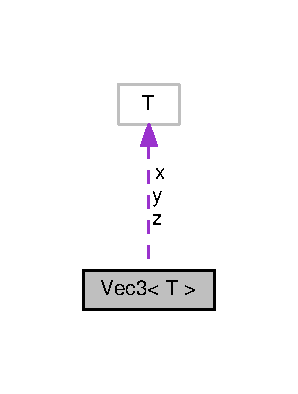
\includegraphics[width=143pt]{structVec3__coll__graph}
\end{center}
\end{figure}
\subsection*{Открытые члены}
\begin{DoxyCompactItemize}
\item 
\mbox{\Hypertarget{structVec3_ab5e07fff614504292d74e3d7f29fe6f9}\label{structVec3_ab5e07fff614504292d74e3d7f29fe6f9}} 
{\bfseries Vec3} (T \+\_\+x, T \+\_\+y, T \+\_\+z)
\item 
\mbox{\Hypertarget{structVec3_abd0f82b0379abee8cea2a2158f3180f1}\label{structVec3_abd0f82b0379abee8cea2a2158f3180f1}} 
\hyperlink{structVec3}{Vec3} \hyperlink{structVec3_abd0f82b0379abee8cea2a2158f3180f1}{operator$^\wedge$} (const \hyperlink{structVec3}{Vec3} \&v) const
\begin{DoxyCompactList}\small\item\em Векторное произведение двух векторов \end{DoxyCompactList}\item 
\mbox{\Hypertarget{structVec3_ab4c15073725c9533bab9949d683de7fa}\label{structVec3_ab4c15073725c9533bab9949d683de7fa}} 
\hyperlink{structVec3}{Vec3} \hyperlink{structVec3_ab4c15073725c9533bab9949d683de7fa}{operator+} (const \hyperlink{structVec3}{Vec3} \&v) const
\begin{DoxyCompactList}\small\item\em Сложение двух векторов \end{DoxyCompactList}\item 
\mbox{\Hypertarget{structVec3_a2d5c95b3111fb791acc763d3fcb9ebec}\label{structVec3_a2d5c95b3111fb791acc763d3fcb9ebec}} 
\hyperlink{structVec3}{Vec3} \hyperlink{structVec3_a2d5c95b3111fb791acc763d3fcb9ebec}{operator-\/} (const \hyperlink{structVec3}{Vec3} \&v) const
\begin{DoxyCompactList}\small\item\em Вычитание двух векторов \end{DoxyCompactList}\item 
\mbox{\Hypertarget{structVec3_a19d8367ca7b06fd84c1d71c36ea798d1}\label{structVec3_a19d8367ca7b06fd84c1d71c36ea798d1}} 
\hyperlink{structVec3}{Vec3} \hyperlink{structVec3_a19d8367ca7b06fd84c1d71c36ea798d1}{operator$\ast$} (T f) const
\begin{DoxyCompactList}\small\item\em Масштабирование вектора \end{DoxyCompactList}\item 
\mbox{\Hypertarget{structVec3_a95f0f9e61705b0985ebb9a428c2b89fc}\label{structVec3_a95f0f9e61705b0985ebb9a428c2b89fc}} 
T \hyperlink{structVec3_a95f0f9e61705b0985ebb9a428c2b89fc}{operator$\ast$} (const \hyperlink{structVec3}{Vec3} \&v) const
\begin{DoxyCompactList}\small\item\em Скалярное произведение двух векторов \end{DoxyCompactList}\item 
\mbox{\Hypertarget{structVec3_af820381ed8bfdb2c82bf8d960b2596b4}\label{structVec3_af820381ed8bfdb2c82bf8d960b2596b4}} 
T \hyperlink{structVec3_af820381ed8bfdb2c82bf8d960b2596b4}{norm} () const
\begin{DoxyCompactList}\small\item\em Длина вектора \end{DoxyCompactList}\item 
\mbox{\Hypertarget{structVec3_a5ac8f4b5ab9b52abfc101b45f39c5c8f}\label{structVec3_a5ac8f4b5ab9b52abfc101b45f39c5c8f}} 
T \& {\bfseries operator\mbox{[}$\,$\mbox{]}} (const int i)
\end{DoxyCompactItemize}
\subsection*{Открытые атрибуты}
\begin{DoxyCompactItemize}
\item 
\mbox{\Hypertarget{structVec3_aeba95c52e15a5a7476550c1798210db2}\label{structVec3_aeba95c52e15a5a7476550c1798210db2}} 
T {\bfseries x}
\item 
\mbox{\Hypertarget{structVec3_a76f06eaf078504ac1d09c910ddb24696}\label{structVec3_a76f06eaf078504ac1d09c910ddb24696}} 
T {\bfseries y}
\item 
\mbox{\Hypertarget{structVec3_a0f694311f956380952aee054cbabb8b6}\label{structVec3_a0f694311f956380952aee054cbabb8b6}} 
T {\bfseries z}
\end{DoxyCompactItemize}
\subsection*{Друзья}
\begin{DoxyCompactItemize}
\item 
\mbox{\Hypertarget{structVec3_acf89f9161224752f03cb423da592035e}\label{structVec3_acf89f9161224752f03cb423da592035e}} 
std\+::ostream \& {\bfseries operator$<$$<$} (std\+::ostream \&s, \hyperlink{structVec3}{Vec3} \&v)
\end{DoxyCompactItemize}


\subsection{Подробное описание}
\subsubsection*{template$<$class T$>$\newline
struct Vec3$<$ T $>$}

Класс 3D вектора 

Объявления и описания членов структуры находятся в файле\+:\begin{DoxyCompactItemize}
\item 
geometry.\+h\end{DoxyCompactItemize}

\hypertarget{classVectorController}{}\section{Класс Vector\+Controller}
\label{classVectorController}\index{Vector\+Controller@{Vector\+Controller}}


Класс векторного контроллера  




{\ttfamily \#include $<$controller.\+h$>$}

\subsection*{Открытые члены}
\begin{DoxyCompactItemize}
\item 
\hyperlink{structVec3}{Vec3d} \hyperlink{classVectorController_a1ec5293a94bd834736e5c6fbf293dbb8}{operator()} (double phi, double refpos, \hyperlink{structVec3}{Vec3d} iabc)
\begin{DoxyCompactList}\small\item\em обновляет сотояние \end{DoxyCompactList}\end{DoxyCompactItemize}


\subsection{Подробное описание}
Класс векторного контроллера 

\subsection{Методы}
\mbox{\Hypertarget{classVectorController_a1ec5293a94bd834736e5c6fbf293dbb8}\label{classVectorController_a1ec5293a94bd834736e5c6fbf293dbb8}} 
\index{Vector\+Controller@{Vector\+Controller}!operator()@{operator()}}
\index{operator()@{operator()}!Vector\+Controller@{Vector\+Controller}}
\subsubsection{\texorpdfstring{operator()()}{operator()()}}
{\footnotesize\ttfamily \hyperlink{structVec3}{Vec3d} Vector\+Controller\+::operator() (\begin{DoxyParamCaption}\item[{double}]{phi,  }\item[{double}]{refpos,  }\item[{\hyperlink{structVec3}{Vec3d}}]{iabc }\end{DoxyParamCaption})\hspace{0.3cm}{\ttfamily [inline]}}



обновляет сотояние 


\begin{DoxyParams}{Аргументы}
{\em phi} & угловое положение ротора рад \\
\hline
{\em refpos} & напряжение уставки контура положения В \\
\hline
{\em iabc} & фазные токи статора А \\
\hline
\end{DoxyParams}
\begin{DoxyReturn}{Возвращает}
вектор фазных напряжений статора В 
\end{DoxyReturn}


Объявления и описания членов класса находятся в файле\+:\begin{DoxyCompactItemize}
\item 
controller.\+h\end{DoxyCompactItemize}

\chapter{Файлы}
\hypertarget{config_8h}{}\section{Файл config.\+h}
\label{config_8h}\index{config.\+h@{config.\+h}}
Граф файлов, в которые включается этот файл\+:\nopagebreak
\begin{figure}[H]
\begin{center}
\leavevmode
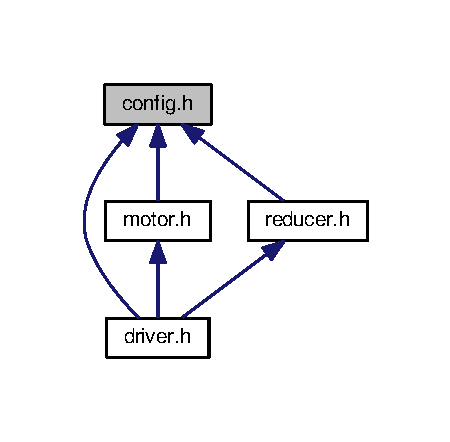
\includegraphics[width=216pt]{config_8h__dep__incl}
\end{center}
\end{figure}
\subsection*{Переменные}
\begin{DoxyCompactItemize}
\item 
const double \hyperlink{config_8h_a88bed2c6a6c301ef59ccb9ed30b34bbe}{P\+S\+I\+M\+AX} =0.\+01121
\item 
const double \hyperlink{config_8h_a8d866ff11caf3e35eafef6778585ff67}{L\+D\+RV} = 152e-\/6
\item 
const double \hyperlink{config_8h_a75d859ba55ae0e14d8b324e1665fb7cf}{R\+D\+RV} = 0.\+9
\item 
const double \hyperlink{config_8h_a3a447872118900d7686c5296e11c7c5b}{N\+P\+OL} = 4
\item 
const double \hyperlink{config_8h_a7e5583efc197d188899a8ea0fb74d842}{J\+D\+RV} = 14e-\/6
\item 
const double \hyperlink{config_8h_adc458bd552568a0145a18009829c6089}{J\+\_\+\+R\+E\+D\+P\+R\+IV} = 1.\+33e-\/6
\item 
const double \hyperlink{config_8h_a54d952ecaf519c3a34657ce012c9ec9e}{K\+\_\+\+S\+T\+R\+DV} = 1.\+778e-\/6
\item 
const double \hyperlink{config_8h_a47837ecd23b1a6f5eed6260498148fea}{M\+\_\+\+S\+T\+R0} = 0.\+005
\item 
const double \hyperlink{config_8h_ad8eb775e11f7df8a694a562de1ba67f1}{K\+\_\+\+V\+T\+R\+DV} = 4.\+52e-\/5
\item 
const double \hyperlink{config_8h_aea0e8a1c248a8a6361f86e9089787291}{I\+\_\+\+R\+ED} = 2e-\/3/2/\+M\+\_\+\+PI
\item 
const double \hyperlink{config_8h_aede2dbe47eaae228feb68e8c82eb1c42}{E\+T\+H\+A\+\_\+T} = 0.\+86
\item 
const double \hyperlink{config_8h_a19abfffecaca8d8589b7c2e3edfbc685}{E\+T\+H\+A\+\_\+\+T\+O\+RM} = 0.\+84
\item 
const double \hyperlink{config_8h_a7b2cd7eb015a69fc1fe7eb10b6659aa7}{D\+E\+L\+T\+A\+\_\+\+R\+ED} = 30e-\/6
\item 
const double \hyperlink{config_8h_a72f587b4f0fd8c365a5cc86b2b074044}{C\+\_\+\+R\+ED} = 1.\+064e8
\item 
const double \hyperlink{config_8h_ad03bcc3f8ad18c90289aef5b4b5fbb6d}{B\+\_\+\+R\+ED} = 150e3
\item 
const double \hyperlink{config_8h_a05533667be853f4591ebffff7fbc2d93}{K\+\_\+N} = 295e3
\item 
const double \hyperlink{config_8h_ad73c100f9562287d3c8e75e5196362c1}{M\+\_\+\+M\+EX} = 9.\+887
\item 
const double \hyperlink{config_8h_a1516697934f71a7a919c7a4110a1af05}{F\+\_\+\+S\+T\+RN} = 480.\+0
\item 
const double \hyperlink{config_8h_a1e8b8bfe82fd2ebb3eee0aa3ed173ded}{K\+\_\+\+V\+T\+RN} = 640.\+0
\item 
const double \hyperlink{config_8h_a04901ad6604d09812173056611c8ac22}{U\+P\+WR} = 57
\end{DoxyCompactItemize}


\subsection{Подробное описание}
Параметры модели 

\subsection{Переменные}
\mbox{\Hypertarget{config_8h_ad03bcc3f8ad18c90289aef5b4b5fbb6d}\label{config_8h_ad03bcc3f8ad18c90289aef5b4b5fbb6d}} 
\index{config.\+h@{config.\+h}!B\+\_\+\+R\+ED@{B\+\_\+\+R\+ED}}
\index{B\+\_\+\+R\+ED@{B\+\_\+\+R\+ED}!config.\+h@{config.\+h}}
\subsubsection{\texorpdfstring{B\+\_\+\+R\+ED}{B\_RED}}
{\footnotesize\ttfamily const double B\+\_\+\+R\+ED = 150e3}


\begin{DoxyParams}{Аргументы}
{\em Коэффициент} & вязкого трения при упругой деформации в редукторе, приведённый к штоку Н$\ast$с/м \\
\hline
\end{DoxyParams}
\mbox{\Hypertarget{config_8h_a72f587b4f0fd8c365a5cc86b2b074044}\label{config_8h_a72f587b4f0fd8c365a5cc86b2b074044}} 
\index{config.\+h@{config.\+h}!C\+\_\+\+R\+ED@{C\+\_\+\+R\+ED}}
\index{C\+\_\+\+R\+ED@{C\+\_\+\+R\+ED}!config.\+h@{config.\+h}}
\subsubsection{\texorpdfstring{C\+\_\+\+R\+ED}{C\_RED}}
{\footnotesize\ttfamily const double C\+\_\+\+R\+ED = 1.\+064e8}


\begin{DoxyParams}{Аргументы}
{\em Коэффициент} & жёсткости редуктора, приведённый к штоку Н/м \\
\hline
\end{DoxyParams}
\mbox{\Hypertarget{config_8h_a7b2cd7eb015a69fc1fe7eb10b6659aa7}\label{config_8h_a7b2cd7eb015a69fc1fe7eb10b6659aa7}} 
\index{config.\+h@{config.\+h}!D\+E\+L\+T\+A\+\_\+\+R\+ED@{D\+E\+L\+T\+A\+\_\+\+R\+ED}}
\index{D\+E\+L\+T\+A\+\_\+\+R\+ED@{D\+E\+L\+T\+A\+\_\+\+R\+ED}!config.\+h@{config.\+h}}
\subsubsection{\texorpdfstring{D\+E\+L\+T\+A\+\_\+\+R\+ED}{DELTA\_RED}}
{\footnotesize\ttfamily const double D\+E\+L\+T\+A\+\_\+\+R\+ED = 30e-\/6}


\begin{DoxyParams}{Аргументы}
{\em Люфт} & редуктора, приведённый к штоку м \\
\hline
\end{DoxyParams}
\mbox{\Hypertarget{config_8h_aede2dbe47eaae228feb68e8c82eb1c42}\label{config_8h_aede2dbe47eaae228feb68e8c82eb1c42}} 
\index{config.\+h@{config.\+h}!E\+T\+H\+A\+\_\+T@{E\+T\+H\+A\+\_\+T}}
\index{E\+T\+H\+A\+\_\+T@{E\+T\+H\+A\+\_\+T}!config.\+h@{config.\+h}}
\subsubsection{\texorpdfstring{E\+T\+H\+A\+\_\+T}{ETHA\_T}}
{\footnotesize\ttfamily const double E\+T\+H\+A\+\_\+T = 0.\+86}


\begin{DoxyParams}{Аргументы}
{\em Коэффициент} & полезного действия планетарного механизма в тяговом режиме \\
\hline
\end{DoxyParams}
\mbox{\Hypertarget{config_8h_a19abfffecaca8d8589b7c2e3edfbc685}\label{config_8h_a19abfffecaca8d8589b7c2e3edfbc685}} 
\index{config.\+h@{config.\+h}!E\+T\+H\+A\+\_\+\+T\+O\+RM@{E\+T\+H\+A\+\_\+\+T\+O\+RM}}
\index{E\+T\+H\+A\+\_\+\+T\+O\+RM@{E\+T\+H\+A\+\_\+\+T\+O\+RM}!config.\+h@{config.\+h}}
\subsubsection{\texorpdfstring{E\+T\+H\+A\+\_\+\+T\+O\+RM}{ETHA\_TORM}}
{\footnotesize\ttfamily const double E\+T\+H\+A\+\_\+\+T\+O\+RM = 0.\+84}


\begin{DoxyParams}{Аргументы}
{\em Коэффициент} & полезного действия планетарного механизма в режиме торможения \\
\hline
\end{DoxyParams}
\mbox{\Hypertarget{config_8h_a1516697934f71a7a919c7a4110a1af05}\label{config_8h_a1516697934f71a7a919c7a4110a1af05}} 
\index{config.\+h@{config.\+h}!F\+\_\+\+S\+T\+RN@{F\+\_\+\+S\+T\+RN}}
\index{F\+\_\+\+S\+T\+RN@{F\+\_\+\+S\+T\+RN}!config.\+h@{config.\+h}}
\subsubsection{\texorpdfstring{F\+\_\+\+S\+T\+RN}{F\_STRN}}
{\footnotesize\ttfamily const double F\+\_\+\+S\+T\+RN = 480.\+0}


\begin{DoxyParams}{Аргументы}
{\em Сила} & сухого трения в исполнительном механизме, приведённая к штоку Н \\
\hline
\end{DoxyParams}
\mbox{\Hypertarget{config_8h_aea0e8a1c248a8a6361f86e9089787291}\label{config_8h_aea0e8a1c248a8a6361f86e9089787291}} 
\index{config.\+h@{config.\+h}!I\+\_\+\+R\+ED@{I\+\_\+\+R\+ED}}
\index{I\+\_\+\+R\+ED@{I\+\_\+\+R\+ED}!config.\+h@{config.\+h}}
\subsubsection{\texorpdfstring{I\+\_\+\+R\+ED}{I\_RED}}
{\footnotesize\ttfamily const double I\+\_\+\+R\+ED = 2e-\/3/2/\+M\+\_\+\+PI}


\begin{DoxyParams}{Аргументы}
{\em Кинематический} & коэффициент передачи редуктора м/рад \\
\hline
\end{DoxyParams}
\mbox{\Hypertarget{config_8h_adc458bd552568a0145a18009829c6089}\label{config_8h_adc458bd552568a0145a18009829c6089}} 
\index{config.\+h@{config.\+h}!J\+\_\+\+R\+E\+D\+P\+R\+IV@{J\+\_\+\+R\+E\+D\+P\+R\+IV}}
\index{J\+\_\+\+R\+E\+D\+P\+R\+IV@{J\+\_\+\+R\+E\+D\+P\+R\+IV}!config.\+h@{config.\+h}}
\subsubsection{\texorpdfstring{J\+\_\+\+R\+E\+D\+P\+R\+IV}{J\_REDPRIV}}
{\footnotesize\ttfamily const double J\+\_\+\+R\+E\+D\+P\+R\+IV = 1.\+33e-\/6}


\begin{DoxyParams}{Аргументы}
{\em Момент} & инерции вращающихся частей редуктора, приведённый к ротору двигателя кг$\ast$м2 \\
\hline
\end{DoxyParams}
\mbox{\Hypertarget{config_8h_a7e5583efc197d188899a8ea0fb74d842}\label{config_8h_a7e5583efc197d188899a8ea0fb74d842}} 
\index{config.\+h@{config.\+h}!J\+D\+RV@{J\+D\+RV}}
\index{J\+D\+RV@{J\+D\+RV}!config.\+h@{config.\+h}}
\subsubsection{\texorpdfstring{J\+D\+RV}{JDRV}}
{\footnotesize\ttfamily const double J\+D\+RV = 14e-\/6}


\begin{DoxyParams}{Аргументы}
{\em Момент} & инерции ротора двигателя кг$\ast$м2 \\
\hline
\end{DoxyParams}
\mbox{\Hypertarget{config_8h_a05533667be853f4591ebffff7fbc2d93}\label{config_8h_a05533667be853f4591ebffff7fbc2d93}} 
\index{config.\+h@{config.\+h}!K\+\_\+N@{K\+\_\+N}}
\index{K\+\_\+N@{K\+\_\+N}!config.\+h@{config.\+h}}
\subsubsection{\texorpdfstring{K\+\_\+N}{K\_N}}
{\footnotesize\ttfamily const double K\+\_\+N = 295e3}


\begin{DoxyParams}{Аргументы}
{\em Коэффициент} & аэродинамической нагрузки, приведённый к штоку Н/м \\
\hline
\end{DoxyParams}
\mbox{\Hypertarget{config_8h_a54d952ecaf519c3a34657ce012c9ec9e}\label{config_8h_a54d952ecaf519c3a34657ce012c9ec9e}} 
\index{config.\+h@{config.\+h}!K\+\_\+\+S\+T\+R\+DV@{K\+\_\+\+S\+T\+R\+DV}}
\index{K\+\_\+\+S\+T\+R\+DV@{K\+\_\+\+S\+T\+R\+DV}!config.\+h@{config.\+h}}
\subsubsection{\texorpdfstring{K\+\_\+\+S\+T\+R\+DV}{K\_STRDV}}
{\footnotesize\ttfamily const double K\+\_\+\+S\+T\+R\+DV = 1.\+778e-\/6}


\begin{DoxyParams}{Аргументы}
{\em Коэффициент} & сухого трения, возникающего при осевом усилии Fупр на подшипники двигателя м \\
\hline
\end{DoxyParams}
\mbox{\Hypertarget{config_8h_ad8eb775e11f7df8a694a562de1ba67f1}\label{config_8h_ad8eb775e11f7df8a694a562de1ba67f1}} 
\index{config.\+h@{config.\+h}!K\+\_\+\+V\+T\+R\+DV@{K\+\_\+\+V\+T\+R\+DV}}
\index{K\+\_\+\+V\+T\+R\+DV@{K\+\_\+\+V\+T\+R\+DV}!config.\+h@{config.\+h}}
\subsubsection{\texorpdfstring{K\+\_\+\+V\+T\+R\+DV}{K\_VTRDV}}
{\footnotesize\ttfamily const double K\+\_\+\+V\+T\+R\+DV = 4.\+52e-\/5}


\begin{DoxyParams}{Аргументы}
{\em Коэффициент} & вязкого трения в подшипниках двигателя Н$\ast$м$\ast$с/рад \\
\hline
\end{DoxyParams}
\mbox{\Hypertarget{config_8h_a1e8b8bfe82fd2ebb3eee0aa3ed173ded}\label{config_8h_a1e8b8bfe82fd2ebb3eee0aa3ed173ded}} 
\index{config.\+h@{config.\+h}!K\+\_\+\+V\+T\+RN@{K\+\_\+\+V\+T\+RN}}
\index{K\+\_\+\+V\+T\+RN@{K\+\_\+\+V\+T\+RN}!config.\+h@{config.\+h}}
\subsubsection{\texorpdfstring{K\+\_\+\+V\+T\+RN}{K\_VTRN}}
{\footnotesize\ttfamily const double K\+\_\+\+V\+T\+RN = 640.\+0}


\begin{DoxyParams}{Аргументы}
{\em Коэффициент} & вязкого трения в исполнительном механизме, приведённый к штоку Н$\ast$с/м \\
\hline
\end{DoxyParams}
\mbox{\Hypertarget{config_8h_a8d866ff11caf3e35eafef6778585ff67}\label{config_8h_a8d866ff11caf3e35eafef6778585ff67}} 
\index{config.\+h@{config.\+h}!L\+D\+RV@{L\+D\+RV}}
\index{L\+D\+RV@{L\+D\+RV}!config.\+h@{config.\+h}}
\subsubsection{\texorpdfstring{L\+D\+RV}{LDRV}}
{\footnotesize\ttfamily const double L\+D\+RV = 152e-\/6}


\begin{DoxyParams}{Аргументы}
{\em L\+D\+RV} & Индуктивность фазы двигателя Гн \\
\hline
\end{DoxyParams}
\mbox{\Hypertarget{config_8h_ad73c100f9562287d3c8e75e5196362c1}\label{config_8h_ad73c100f9562287d3c8e75e5196362c1}} 
\index{config.\+h@{config.\+h}!M\+\_\+\+M\+EX@{M\+\_\+\+M\+EX}}
\index{M\+\_\+\+M\+EX@{M\+\_\+\+M\+EX}!config.\+h@{config.\+h}}
\subsubsection{\texorpdfstring{M\+\_\+\+M\+EX}{M\_MEX}}
{\footnotesize\ttfamily const double M\+\_\+\+M\+EX = 9.\+887}


\begin{DoxyParams}{Аргументы}
{\em Масса} & исполнительного механизма, приведённая к штоку кг \\
\hline
\end{DoxyParams}
\mbox{\Hypertarget{config_8h_a47837ecd23b1a6f5eed6260498148fea}\label{config_8h_a47837ecd23b1a6f5eed6260498148fea}} 
\index{config.\+h@{config.\+h}!M\+\_\+\+S\+T\+R0@{M\+\_\+\+S\+T\+R0}}
\index{M\+\_\+\+S\+T\+R0@{M\+\_\+\+S\+T\+R0}!config.\+h@{config.\+h}}
\subsubsection{\texorpdfstring{M\+\_\+\+S\+T\+R0}{M\_STR0}}
{\footnotesize\ttfamily const double M\+\_\+\+S\+T\+R0 = 0.\+005}


\begin{DoxyParams}{Аргументы}
{\em Постоянная} & составляющая момента сухого трения ротора двигателя Н$\ast$м \\
\hline
\end{DoxyParams}
\mbox{\Hypertarget{config_8h_a3a447872118900d7686c5296e11c7c5b}\label{config_8h_a3a447872118900d7686c5296e11c7c5b}} 
\index{config.\+h@{config.\+h}!N\+P\+OL@{N\+P\+OL}}
\index{N\+P\+OL@{N\+P\+OL}!config.\+h@{config.\+h}}
\subsubsection{\texorpdfstring{N\+P\+OL}{NPOL}}
{\footnotesize\ttfamily const double N\+P\+OL = 4}


\begin{DoxyParams}{Аргументы}
{\em Число} & пар полюсов ротора двигателя \\
\hline
\end{DoxyParams}
\mbox{\Hypertarget{config_8h_a88bed2c6a6c301ef59ccb9ed30b34bbe}\label{config_8h_a88bed2c6a6c301ef59ccb9ed30b34bbe}} 
\index{config.\+h@{config.\+h}!P\+S\+I\+M\+AX@{P\+S\+I\+M\+AX}}
\index{P\+S\+I\+M\+AX@{P\+S\+I\+M\+AX}!config.\+h@{config.\+h}}
\subsubsection{\texorpdfstring{P\+S\+I\+M\+AX}{PSIMAX}}
{\footnotesize\ttfamily const double P\+S\+I\+M\+AX =0.\+01121}


\begin{DoxyParams}{Аргументы}
{\em P\+S\+I\+M\+AX} & Амплитуда потокосцепления, создаваемого постоянными магнитами в обмотках статора Вб \\
\hline
\end{DoxyParams}
\mbox{\Hypertarget{config_8h_a75d859ba55ae0e14d8b324e1665fb7cf}\label{config_8h_a75d859ba55ae0e14d8b324e1665fb7cf}} 
\index{config.\+h@{config.\+h}!R\+D\+RV@{R\+D\+RV}}
\index{R\+D\+RV@{R\+D\+RV}!config.\+h@{config.\+h}}
\subsubsection{\texorpdfstring{R\+D\+RV}{RDRV}}
{\footnotesize\ttfamily const double R\+D\+RV = 0.\+9}


\begin{DoxyParams}{Аргументы}
{\em R\+D\+RV} & Активное сопротивление фазы двигателя Ом \\
\hline
\end{DoxyParams}
\mbox{\Hypertarget{config_8h_a04901ad6604d09812173056611c8ac22}\label{config_8h_a04901ad6604d09812173056611c8ac22}} 
\index{config.\+h@{config.\+h}!U\+P\+WR@{U\+P\+WR}}
\index{U\+P\+WR@{U\+P\+WR}!config.\+h@{config.\+h}}
\subsubsection{\texorpdfstring{U\+P\+WR}{UPWR}}
{\footnotesize\ttfamily const double U\+P\+WR = 57}


\begin{DoxyParams}{Аргументы}
{\em Напряжение} & питания инвертора В \\
\hline
\end{DoxyParams}

\hypertarget{gdef_8h}{}\section{Файл gdef.\+h}
\label{gdef_8h}\index{gdef.\+h@{gdef.\+h}}
Граф файлов, в которые включается этот файл\+:\nopagebreak
\begin{figure}[H]
\begin{center}
\leavevmode
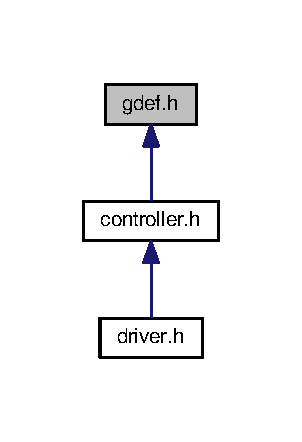
\includegraphics[width=145pt]{gdef_8h__dep__incl}
\end{center}
\end{figure}
\subsection*{Макросы}
\begin{DoxyCompactItemize}
\item 
\#define \hyperlink{gdef_8h_a52badf88bc1d7d2b1a36d9c65cba4514}{K\+I\+\_\+\+D\+Q\+C\+UR}~400
\item 
\#define \hyperlink{gdef_8h_ae7a7147dbc94a7c2f929f30185b28d1b}{K\+P\+\_\+\+D\+Q\+C\+UR}~1000
\item 
\#define \hyperlink{gdef_8h_a80b1a98f2d512a1faf0c9ae8b0341678}{K\+I\+\_\+\+S\+PD}~0
\item 
\#define \hyperlink{gdef_8h_afea6c55d490722ff4dd28b9845377372}{K\+P\+\_\+\+S\+PD}~9000
\item 
\#define \hyperlink{gdef_8h_a44a89d57c201b8677a6870a86938e578}{K\+I\+\_\+\+P\+OS}~50
\item 
\#define \hyperlink{gdef_8h_add99248873d47589774c628f2fc47530}{K\+P\+\_\+\+P\+OS}~13000
\item 
\#define \hyperlink{gdef_8h_a9f8e58ff97c46154724cbca9cc12bc6a}{M\+A\+X\+Q\+C\+U\+R\+R\+E\+NT}~2000
\item 
\#define \hyperlink{gdef_8h_a7e49c0004749dd2461e791b4c4a97895}{M\+A\+X\+S\+P\+E\+ED}~10000
\item 
\#define \hyperlink{gdef_8h_a663eb72f2c34d68e830ad1ea14938850}{M\+A\+X\+P\+WM}~512
\end{DoxyCompactItemize}


\subsection{Подробное описание}
Параметры векторного контроллера 

\subsection{Макросы}
\mbox{\Hypertarget{gdef_8h_a52badf88bc1d7d2b1a36d9c65cba4514}\label{gdef_8h_a52badf88bc1d7d2b1a36d9c65cba4514}} 
\index{gdef.\+h@{gdef.\+h}!K\+I\+\_\+\+D\+Q\+C\+UR@{K\+I\+\_\+\+D\+Q\+C\+UR}}
\index{K\+I\+\_\+\+D\+Q\+C\+UR@{K\+I\+\_\+\+D\+Q\+C\+UR}!gdef.\+h@{gdef.\+h}}
\subsubsection{\texorpdfstring{K\+I\+\_\+\+D\+Q\+C\+UR}{KI\_DQCUR}}
{\footnotesize\ttfamily \#define K\+I\+\_\+\+D\+Q\+C\+UR~400}


\begin{DoxyParams}{Аргументы}
{\em Интегральная} & составляющая регулятора токов \\
\hline
\end{DoxyParams}
\mbox{\Hypertarget{gdef_8h_a44a89d57c201b8677a6870a86938e578}\label{gdef_8h_a44a89d57c201b8677a6870a86938e578}} 
\index{gdef.\+h@{gdef.\+h}!K\+I\+\_\+\+P\+OS@{K\+I\+\_\+\+P\+OS}}
\index{K\+I\+\_\+\+P\+OS@{K\+I\+\_\+\+P\+OS}!gdef.\+h@{gdef.\+h}}
\subsubsection{\texorpdfstring{K\+I\+\_\+\+P\+OS}{KI\_POS}}
{\footnotesize\ttfamily \#define K\+I\+\_\+\+P\+OS~50}


\begin{DoxyParams}{Аргументы}
{\em Интегральная} & составляющая регулятора положения \\
\hline
\end{DoxyParams}
\mbox{\Hypertarget{gdef_8h_a80b1a98f2d512a1faf0c9ae8b0341678}\label{gdef_8h_a80b1a98f2d512a1faf0c9ae8b0341678}} 
\index{gdef.\+h@{gdef.\+h}!K\+I\+\_\+\+S\+PD@{K\+I\+\_\+\+S\+PD}}
\index{K\+I\+\_\+\+S\+PD@{K\+I\+\_\+\+S\+PD}!gdef.\+h@{gdef.\+h}}
\subsubsection{\texorpdfstring{K\+I\+\_\+\+S\+PD}{KI\_SPD}}
{\footnotesize\ttfamily \#define K\+I\+\_\+\+S\+PD~0}


\begin{DoxyParams}{Аргументы}
{\em Интегральная} & составляющая регулятора скорости \\
\hline
\end{DoxyParams}
\mbox{\Hypertarget{gdef_8h_ae7a7147dbc94a7c2f929f30185b28d1b}\label{gdef_8h_ae7a7147dbc94a7c2f929f30185b28d1b}} 
\index{gdef.\+h@{gdef.\+h}!K\+P\+\_\+\+D\+Q\+C\+UR@{K\+P\+\_\+\+D\+Q\+C\+UR}}
\index{K\+P\+\_\+\+D\+Q\+C\+UR@{K\+P\+\_\+\+D\+Q\+C\+UR}!gdef.\+h@{gdef.\+h}}
\subsubsection{\texorpdfstring{K\+P\+\_\+\+D\+Q\+C\+UR}{KP\_DQCUR}}
{\footnotesize\ttfamily \#define K\+P\+\_\+\+D\+Q\+C\+UR~1000}


\begin{DoxyParams}{Аргументы}
{\em Пропорциональная} & составляющая регулятора токов \\
\hline
\end{DoxyParams}
\mbox{\Hypertarget{gdef_8h_add99248873d47589774c628f2fc47530}\label{gdef_8h_add99248873d47589774c628f2fc47530}} 
\index{gdef.\+h@{gdef.\+h}!K\+P\+\_\+\+P\+OS@{K\+P\+\_\+\+P\+OS}}
\index{K\+P\+\_\+\+P\+OS@{K\+P\+\_\+\+P\+OS}!gdef.\+h@{gdef.\+h}}
\subsubsection{\texorpdfstring{K\+P\+\_\+\+P\+OS}{KP\_POS}}
{\footnotesize\ttfamily \#define K\+P\+\_\+\+P\+OS~13000}


\begin{DoxyParams}{Аргументы}
{\em Пропорциональная} & составляющая регулятора положения \\
\hline
\end{DoxyParams}
\mbox{\Hypertarget{gdef_8h_afea6c55d490722ff4dd28b9845377372}\label{gdef_8h_afea6c55d490722ff4dd28b9845377372}} 
\index{gdef.\+h@{gdef.\+h}!K\+P\+\_\+\+S\+PD@{K\+P\+\_\+\+S\+PD}}
\index{K\+P\+\_\+\+S\+PD@{K\+P\+\_\+\+S\+PD}!gdef.\+h@{gdef.\+h}}
\subsubsection{\texorpdfstring{K\+P\+\_\+\+S\+PD}{KP\_SPD}}
{\footnotesize\ttfamily \#define K\+P\+\_\+\+S\+PD~9000}


\begin{DoxyParams}{Аргументы}
{\em Пропорциональная} & составляющая регулятора скорости \\
\hline
\end{DoxyParams}
\mbox{\Hypertarget{gdef_8h_a663eb72f2c34d68e830ad1ea14938850}\label{gdef_8h_a663eb72f2c34d68e830ad1ea14938850}} 
\index{gdef.\+h@{gdef.\+h}!M\+A\+X\+P\+WM@{M\+A\+X\+P\+WM}}
\index{M\+A\+X\+P\+WM@{M\+A\+X\+P\+WM}!gdef.\+h@{gdef.\+h}}
\subsubsection{\texorpdfstring{M\+A\+X\+P\+WM}{MAXPWM}}
{\footnotesize\ttfamily \#define M\+A\+X\+P\+WM~512}


\begin{DoxyParams}{Аргументы}
{\em ограничение} & скважности для ШИМ \mbox{[}0-\/512\mbox{]} \\
\hline
\end{DoxyParams}
\mbox{\Hypertarget{gdef_8h_a9f8e58ff97c46154724cbca9cc12bc6a}\label{gdef_8h_a9f8e58ff97c46154724cbca9cc12bc6a}} 
\index{gdef.\+h@{gdef.\+h}!M\+A\+X\+Q\+C\+U\+R\+R\+E\+NT@{M\+A\+X\+Q\+C\+U\+R\+R\+E\+NT}}
\index{M\+A\+X\+Q\+C\+U\+R\+R\+E\+NT@{M\+A\+X\+Q\+C\+U\+R\+R\+E\+NT}!gdef.\+h@{gdef.\+h}}
\subsubsection{\texorpdfstring{M\+A\+X\+Q\+C\+U\+R\+R\+E\+NT}{MAXQCURRENT}}
{\footnotesize\ttfamily \#define M\+A\+X\+Q\+C\+U\+R\+R\+E\+NT~2000}


\begin{DoxyParams}{Аргументы}
{\em ограничение} & для регулятора тока \\
\hline
\end{DoxyParams}
\mbox{\Hypertarget{gdef_8h_a7e49c0004749dd2461e791b4c4a97895}\label{gdef_8h_a7e49c0004749dd2461e791b4c4a97895}} 
\index{gdef.\+h@{gdef.\+h}!M\+A\+X\+S\+P\+E\+ED@{M\+A\+X\+S\+P\+E\+ED}}
\index{M\+A\+X\+S\+P\+E\+ED@{M\+A\+X\+S\+P\+E\+ED}!gdef.\+h@{gdef.\+h}}
\subsubsection{\texorpdfstring{M\+A\+X\+S\+P\+E\+ED}{MAXSPEED}}
{\footnotesize\ttfamily \#define M\+A\+X\+S\+P\+E\+ED~10000}


\begin{DoxyParams}{Аргументы}
{\em ограничение} & для регулятора скорости об/мин \\
\hline
\end{DoxyParams}

%--- End generated contents ---

% Index
\backmatter
\newpage
\phantomsection
\clearemptydoublepage
\addcontentsline{toc}{chapter}{Алфавитный указатель}
\printindex

\end{document}
